% ==============================================================
% APPENDIX
% ==============================================================

\section{Workflow Internals}
\label{app:workflows}

Figures~\ref{fig:appwf1}--\ref{fig:appwf4} show the internal structure of each workflow.

\begin{figure*}[h]
    \centering
    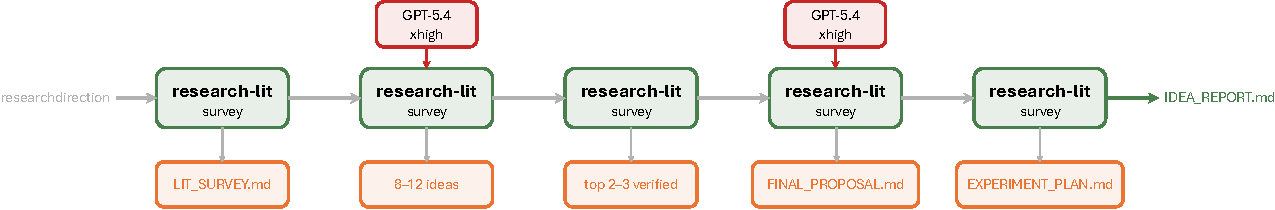
\includegraphics[width=0.95\textwidth]{figures/srcs/10_appwf1.pdf}
    \caption{Workflow~1: Idea Discovery. The pipeline surveys literature, brainstorms ideas via cross-model generation, verifies novelty, and refines the top proposal through iterative GPT-5.4 review.}
    \label{fig:appwf1}
\end{figure*}


\begin{figure*}[h]
    \centering
    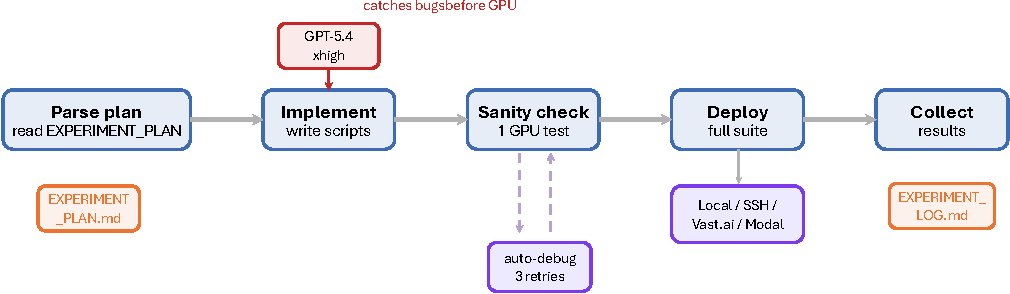
\includegraphics[width=0.95\textwidth]{figures/srcs/11_appwf15.pdf}
    \caption{Workflow~1.5: Experiment Bridge. Scripts are implemented, reviewed for code correctness, sanity-checked on one GPU, then deployed to the full backend.}
    \label{fig:appwf15}
\end{figure*}


\begin{figure*}[h]
    \centering
    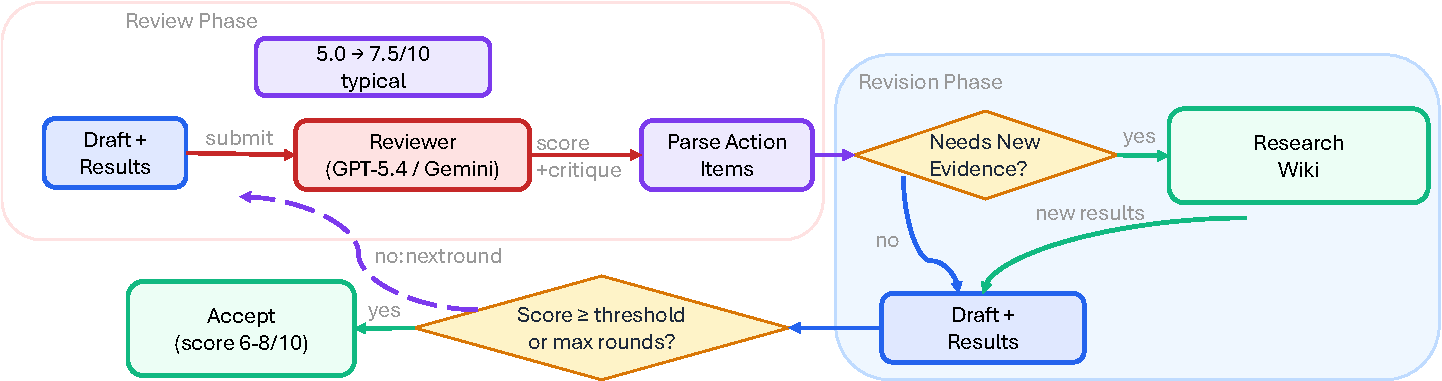
\includegraphics[width=0.95\textwidth]{figures/srcs/06_wf2.pdf}
    \caption{Workflow~2: Auto Review Loop. The reviewer scores the manuscript, the executor implements fixes and runs requested experiments, and the cycle repeats.}
    \label{fig:appwf2}
\end{figure*}

\begin{figure*}[h]
    \centering
    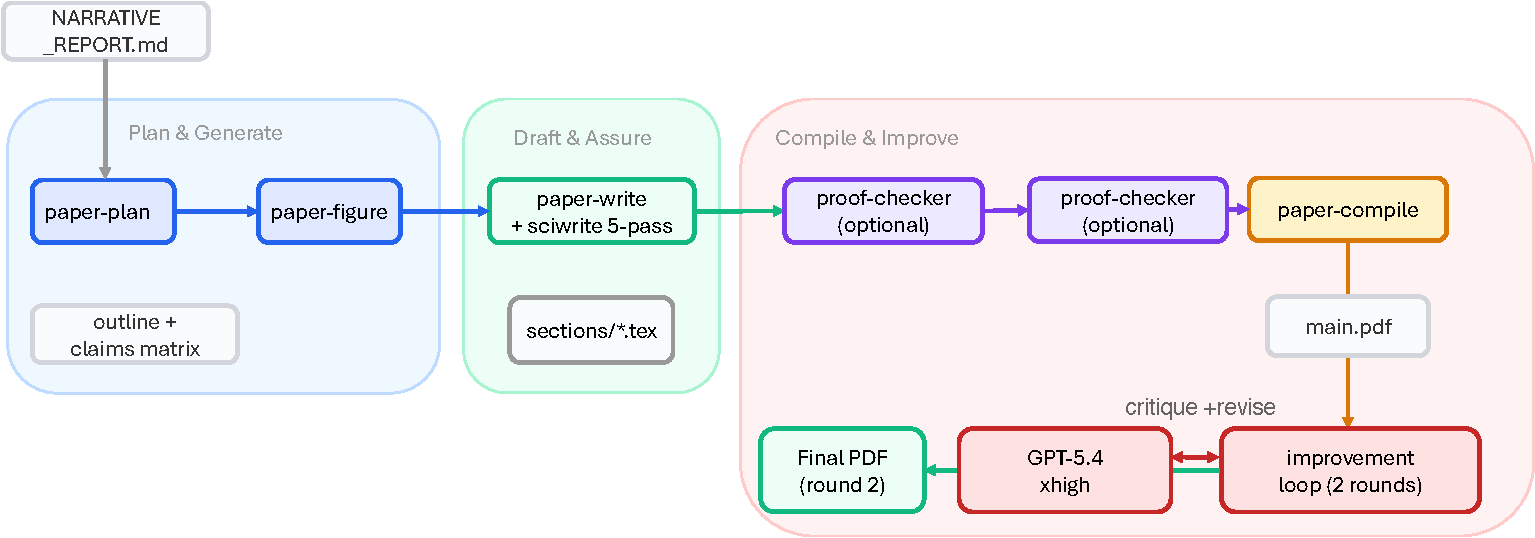
\includegraphics[width=0.95\textwidth]{figures/srcs/07_wf3.pdf}
    \caption{Workflow~3: Paper Writing Pipeline. Seven core sub-skills (plus optional proof checking) chain from outline through figure generation, \LaTeX{} drafting, claim auditing, compilation, and review.}
    \label{fig:appwf3}
\end{figure*}

\begin{figure*}[h]
    \centering
    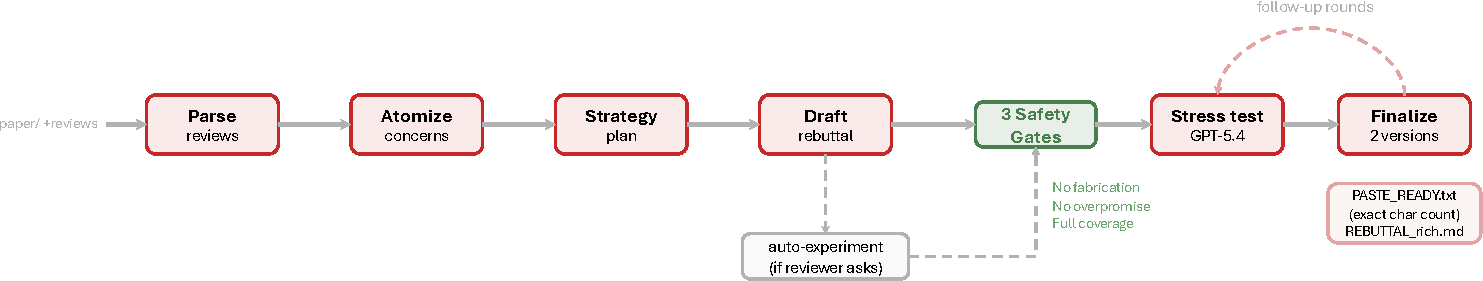
\includegraphics[width=0.95\textwidth]{figures/srcs/12_appwf4.pdf}
    \caption{Workflow~4: Rebuttal. Seven phases from parsing reviews through stress-testing, with three safety gates.}
    \label{fig:appwf4}
\end{figure*}


% ==============================================================
\section{Skill Inventory}
\label{app:skills}

Table~\ref{tab:fullinventory} lists core framework skills in the current release.

\begin{table*}[h]
\centering
\caption{Core \aris{} skill inventory (v0.4, April 2026). Community-contributed skills (30+) are omitted for brevity.}
\label{tab:fullinventory}
\footnotesize
\resizebox{\textwidth}{!}{%
\begin{tabular}{@{}llll@{}}
\toprule
\textbf{Skill} & \textbf{Category} & \textbf{Reviewer?} & \textbf{Key Function} \\
\midrule
\texttt{research-lit} & Literature & No & Multi-source literature survey \\
\texttt{arxiv} / \texttt{alphaxiv} & Literature & No & Paper metadata / LLM-optimized summary \\
\texttt{deepxiv} & Literature & No & Progressive deep literature search \\
\texttt{novelty-check} & Literature & Yes & Novelty verification against existing work \\
\texttt{idea-creator} & Ideation & Yes & Brainstorm and rank research ideas \\
\texttt{idea-discovery} & Ideation & Yes & Full idea discovery pipeline \\
\texttt{experiment-bridge} & Experiment & Yes & Plan to running code \\
\texttt{run-experiment} & Experiment & No & GPU deployment (local/SSH/Vast.ai/Modal) \\
\texttt{monitor-experiment} & Experiment & No & Experiment monitoring and result collection \\
\texttt{check-gpu} & Experiment & No & GPU status and process summary \\
\texttt{analyze-results} & Analysis & No & Statistical analysis and comparison tables \\
\texttt{ablation-planner} & Analysis & No & Reviewer-perspective ablation design \\
\texttt{experiment-audit} & Integrity & Yes & Evaluation code integrity verification \\
\texttt{result-to-claim} & Integrity & No & Result-to-claim verdict conversion \\
\texttt{paper-claim-audit} & Integrity & Yes & Zero-context manuscript number audit \\
\texttt{proof-checker} & Integrity & No & 20-category theorem verification \\
\texttt{auto-review-loop} & Review & Yes & Multi-round autonomous review \\
\texttt{research-review} & Review & Yes & GPT-5.4 xhigh deep critique \\
\texttt{paper-plan} & Writing & Yes & Structural outline + claims matrix \\
\texttt{paper-write} & Writing & Yes & Section-by-section \LaTeX{} + sciwrite 5-pass \\
\texttt{paper-figure} & Writing & No & Publication-quality data plots \\
\texttt{paper-compile} & Writing & No & Multi-pass compilation with auto-repair \\
\texttt{paper-writing} & Writing & Yes & Full W3 pipeline orchestrator \\
\texttt{auto-paper-improvement-loop} & Writing & Yes & Review + visual PDF + auto-revision \\
\texttt{rebuttal} & Writing & Yes & 7-phase rebuttal with safety gates \\
\texttt{research-wiki} & Memory & No & Persistent knowledge base management \\
\texttt{meta-optimize} & Maintenance & Yes & Outer-loop harness optimization \\
\bottomrule
\end{tabular}%
}
\end{table*}

% ==============================================================
\section{Reviewer Configuration}
\label{app:review}

\aris{} configures reviewer behavior along two orthogonal axes (Section~\ref{sec:adversarial}). Table~\ref{tab:scope} lists the three access-scope settings; Table~\ref{tab:context} lists the two context-policy settings.

\begin{table}[h]
\centering
\caption{Reviewer access-scope settings (what the reviewer is allowed to read).}
\label{tab:scope}
\small
\begin{tabular}{@{}lp{8cm}@{}}
\toprule
\textbf{Scope} & \textbf{Description} \\
\midrule
Document-only & Reviewer reads only the manuscript text. Default for paper-writing review. \\
Artifact-augmented & Reviewer additionally reads result files, claim ledgers, and intermediate artifacts referenced by the manuscript. \\
Repository-level & Reviewer directly inspects the codebase, evaluation scripts, and generated outputs through host-provided repository access tools (e.g., \texttt{claude-code} Bash, \texttt{codex exec}). Used by \texttt{experiment-audit} and \texttt{paper-claim-audit}. \\
\bottomrule
\end{tabular}
\end{table}

\begin{table}[h]
\centering
\caption{Reviewer context-policy settings (whether the reviewer retains state across rounds).}
\label{tab:context}
\small
\begin{tabular}{@{}lp{8cm}@{}}
\toprule
\textbf{Policy} & \textbf{Description} \\
\midrule
Fresh & Each review round opens a new reviewer thread with no prior context. Used to prevent confirmation bias from previous rounds (\texttt{REVIEWER\_BIAS\_GUARD = true} default). Required for \texttt{paper-claim-audit} and the auto-paper improvement loop. \\
Cross-round & Reviewer retains memory across rounds, can reference previous critiques and verify whether raised issues have been addressed. Used selectively when convergence verification is more important than independence. \\
\bottomrule
\end{tabular}
\end{table}

% ==============================================================
\section{ARIS-Code Details}
\label{app:ariscode}

\ariscode{} is a standalone Rust-based CLI built on \texttt{claw-code}~\citep{ultraworkers2025}.
Key features: interactive REPL with setup wizard, all skills as slash commands, five LLM providers, native \texttt{LlmReview} tool, three-tier skill priority system (user $>$ Claude Code $>$ bundled), and \texttt{/cost} for token tracking.

% ==============================================================
\section{Controlled Benchmark Protocol (Future Work)}
\label{app:benchmark}

We outline a benchmark protocol for future controlled evaluation:
\textbf{Task pool}: 12+ paper drafts from publicly available preprints.
\textbf{Conditions} (compute-matched): (A)~single-model self-critique, (B)~same-model two-agent, (C)~cross-model, (D)~cross-model reversed, (E)~same-model for the second model.
\textbf{Metrics}: issue recall, false-positive rate, actionability score, downstream revision quality, cost, latency.
\textbf{Raters}: three independent, blinded. Inter-rater agreement via Krippendorff's $\alpha$.
